 \documentclass[]{report}
%\documentclass[10pt,a4paper,headinclude=true,twoside]{report}
\usepackage[latin1]{inputenc}
\usepackage[a4paper]{geometry}
\usepackage{a4wide}
\usepackage{amsmath}
\usepackage{amsfonts}
\usepackage{amssymb}
\usepackage{graphicx}
\usepackage{hyperref}
\usepackage{pdflscape} % dlia landscape orientation 
\hypersetup{colorlinks,citecolor=black,filecolor=black,linkcolor=black,urlcolor=black}
\usepackage{float}
\usepackage{setspace}
\usepackage{titlesec}


\begin{document}
%\onehalfspacing
\title{CS31310: Process for project}
\author{Edgar Ivanov\\ edi@aber.ac.uk \\ Department of Computer Science, Aberystwyth University}
\date{\today}
\maketitle
\section*{Project outline}
My final year project will contain both hardware and software parts. The aim of the project is to build an additional unit which will ensure that camera mounted on the rover is always in a stable position. Currently there is a Pan-and-Tilt Unit (PTU) which controls the camera. It uses gyroscopes to acquire the current position in the space and then adjusts the position of the camera. However gyroscopes are not perfect and tend to drift over time, as well as providing wrong data at the different temperatures. 

I will be building an additional unit which will acquire current position using the more accurate accelerometer and will then provide the PTU with the calibration data.

\section*{Process}
At the moment it is difficult for me to choose the right development methodology for my project. There are a few of them and I have very limited experience of using any of them. Since I didn't go into too much details of my project yet, it will be a bit of guess work to try and find the suitable methodology.

Essentially my customer will be my project supervisor, because I am building the system for him and he is deeply interested in the project. There will be no team of developers working on the project, just me, but I will get the help from my supervisor. The final goal of the project is clear and doesn't seem to be difficult to achieve, so it should be a matter of requirement analysis, design and implementation.

On the other hand, I have very limited knowledge of C programming language and experience of working with proposed hardware. It will be an exploratory work for me as well: finding out how to fit all the parts together and make them work. I may not be able to predict all the pitfalls on the course of the project and as such may need to revise and alter my plan. Having said that I need a flexible methodology, which allows for changes in requirements and design to be made during the development. 

The first thought was to adopt XP with some changes. It was attractive since it didn't require BDUF, documentation, requirements analysis and I could start coding straight away. The problem here would be with pair programming which I believe (after reading why XP is like a ring of poisonous snakes) is compulsory for XP. If there is no design, it is important for somebody to sit next to you and double check all you do to catch the design errors and this would not be possible on a single person project. On-site customer is my next concern, I doubt my supervisor will be able to devote more than a few hours a week for this project, so I can't even speak about the customer being part of the development team, who is essential to make sure that final system meets customer expectations.

I have also thought of waterfall model. I like to have some plan which I can follow. However, I'll have to make changes during the project and waterfall wouldn't be suitable. Spiral model was also considered, but after the deeper reading I found out that it might not be suitable for the smaller projects.

I carried out some more research and decided to try and adapt the evolutionary prototyping model. The prototype system will be built in the beginning. During the course of the project I will then be improving it according to the supervisor's feedback, so that at the end it evolves in to the complete system. I might use a throw-away prototyping model in the beginning to better understand the system requirements and then switch to the evolutionary prototyping, so that it would become a mix of the two life-cycle methodologies. Figure~\ref{fig:Evolutionary_Prototyping} lists the activities of the software development process for the prototyping model. 

\begin{figure}[H]
\centering
\centerline{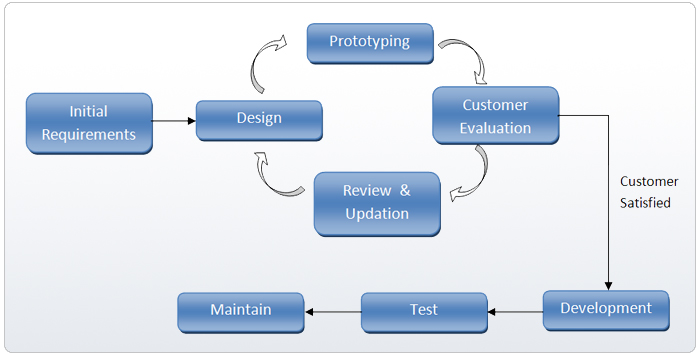
\includegraphics[scale=0.55]{./prototype_methodology}}
\caption{Prototyping model \cite{Evolutionary_Prototyping}}
\label{fig:Evolutionary_Prototyping}
\end{figure}

Requirements are gathered at the beginning, then design is conducted and prototype model is built. Prototype is then evaluated by the customer and feedback is considered at the review \& update stage. If the customer is satisfied with the prototype system it evolves in to the final product. 

I think prototyping methodology will perfectly suit my needs. It is intended to be used when the system is not completely understood by the developer. It will also allow to experiment with various design solutions. The whole project will be split into the smaller segments providing more ease-of-change during the development process. 

\bibliographystyle{ieeetr}
\bibliography{bibl}
\end{document}